% \hypertarget{conclusion}{%
% \section{Conclusion}\label{conclusion}}

\chapter{Conclusion}
\markboth{CONCLUSION}{}
\label{chap:conclusion}
\begin{flushright}
\singlespacing
\emph{``Good judgment depends mostly on experience, and\\ experience usually comes from poor judgment"} \\- Anonymous\footnote{The origin of this frequently misattributed aphorism is unknown \url{https://quoteinvestigator.com/2017/02/23/judgment/}}
\end{flushright}
\onehalfspacing
\vspace{1cm}

% \todo{Actually write a conclusion}

% \section{Synthesis}\label{sec:synthesis}
% \section{Outlook}\label{sec:outlook}
% \section{Afterword}\label{sec:afterword}
% \section*{Gratitude}\label{sec:gratitude}
% \addcontentsline{toc}{section}{Gratitude}

% % Pick a good-looking drop cap https://www.fontsplace.com/free/images/t/typographer-caps_font_preview_characters.gif
	 

	 % https://journals.aps.org/rmp/abstract/10.1103/RevModPhys.90.025008
	 % https://jila.colorado.edu/~junye/yelabsOLD/pubs/scienceArticles/2007/sArticle_2007_10_Helium_DFCS_EPJD.pdf

\section*{Summary of findings}
% \addcontentsline{toc}{section}{Summary of findings}  
	{The} central element of this thesis was helium-4, cast as the workhorse for the experiments for the twin reasons of structural simplicity and unique affordance of three-dimensional single-particle momentum measurements.
	The dominant theme of this dissertation,  metrology, concerns the precision measurement of basic physical quantities to empirically ground present and future theories of physics and was the focus of chapters \ref{chap:transitions} and \ref{chap:tuneout}. 
	These works were motivated by the suitability of the (deceptively) simple helium atom to high-precision calculations.
	In the counterpoint, many-body physics, we turned attention outside the helium atom itself, towards the collective behaviour of interacting particles.
	This theme was elaborated in chapter \ref{chap:QD} (and appendix\ref{chap:lattice}) with particular emphasis on the scientific contributions made possible by `momentum microscopy' of quantum gases.

	Chapter \ref{chap:transitions} presented the first measurement of the spin-forbidden $2\triplet P_2\rightarrow 5\singlet D_2$ line in helium along with new measurements of transitions from the $2\triplet P_2$ state to the $5\triplet S_1$ and $5\triplet D_J~(J\in\{1,2,3\})$ states. 
	These measurements were made by disturbing an optical cooling process during the BEC production sequence, wherein the upper state of the 1083 nm cooling transition served as the lower state for the target transition. 
	When atoms were excited by the cooling light, they were able to absorb resonant probe light and thus degrade the phase-space density of the atomic sample by either absorbing the energy (heating the sample) or decaying to an untrapped state (reducing the number density).
	Subsequently, when the evaporative cooling process amplified the phase space density, the perturbation in the initial condition resulted in a decrease in the total number of atoms cooled to degeneracy.
	As far as I know, this is the first use of such a technique for atomic spectroscopy.
	Other transition measurements are usually made by probing the trapped ground state \cite{Thomas20,Rengelink18,Notermans14}, rather than excited states.
	The resulting determinations of transition frequencies improve upon previous measurements, where they exist \cite{Martin60}, by at least an order of magnitude in precision and are consistent with state-of-the art theoretical predictions.
	However, the precision of this measurement was limited to the level of a few MHz by the wavemeter we employed as the frequency reference.
	In comparison, the uncertainty of theoretical predictions for these transitions is dominated by the 700 kHz uncertainty in the lower state energy.
	The use of a frequency comb locked to a stable frequency reference would be the major instrumental requirement toward challenging the precision of current atomic structure theory calculations - additional considerations are discussed at the end of the chapter.
	


	



	% Such measurements would help constrain the energy of the $2\triplet P_2$ state because, thanks to the $1/n^3$-like scaling of QED uncertainties, theoretical uncertainty in the $n=5$ levels is as low as 
	 % mean the $n=5$ states are known with a factor $\sim5$ better accuracy than the $n=3$ levels, thus bolstering the efforts to understand the 7.4$\sigma$ anomaly in the $n=3$ singlet-triplet level in $^3$He, which has not been measured in $^4$He \cite{Derouard80,Morton06}.

	The content of chapter \ref{chap:tuneout} was a variation on the theme of frequency measurement, focusing instead on the $\TO$ tune-out frequency.
	This measurement was underpinned by a novel technique for trap freqency measurement that yields a single-shot determination of the trapping frequencies with accuracy at the level of tens of ppm.
	This technique was employed to detect the shift in the net trapping frequency of a hybrid magnetic- and optical-dipole trap as a function of the probe laser frequency, and improved on the precision of the ANU group's previous measurement \cite{Henson15} by a factor of 15.
	A further advance over the prior work was made by characterizing the polarization-dependence of the tune-out, eliminating any dependence on parameters which were not precisely measurable and permitting an unambiguous comparison with theory.
	The experimental determination of $725,736,700(40_\mathrm{stat})(260_\mathrm{sys})$ MHz differs from the theoretical prediction of 725,736,053(9) MHz by 2.5$\sigma$, where the experimental accuracy is limited by the imprecise knowledge of the exact polarization of the probe laser light at the atoms.
	This measurement is the first tune-out measurement to resolve corrections for finite-wavelength retardation effects and yields the most precise constraint on the ratio of transition dipole matrix elements in any neutral atom to date.
	Furthermore, the highly accurate trap frequency measurements meant that our longest data collection run at a fixed polarization would be capable of detecting, with an SNR of 1, a differential Stark shift at the level of $10^{-35}$ J.


	In appendix \ref{chap:lattice} I recount the major milestones I achieved towards the construction of a new BEC machine with the objective of trapping \mhe~atoms in a 3D optical lattice.
	Over the course of work on this project, I built the vacuum system, the optomechanical and optoelectronic systems used to control and distribute laser light for cooling, trapping and imaging applications, and the imaging system (including hardware assembly and attendant software suite), all of which are still in use in the laboratory.
	This lab has since gone on to achieve condensation of $^4$He in a record time of only 3.3 seconds, with very large condensed populations on the order of a million atoms \cite{Abbas21}.
	Work towards the operation of the optical lattice is ongoing.

	Finally, the topic of chapter \ref{chap:QD} was the physics of the condensed state itself.
	This work concerned the density measurements of the ultra-dilute, large-momentum halo around the condensate and outside the thermal fraction.
	In this region of momentum space, we found evidence suggestive of the persistence of the quantum depletion through the expansion into the far-field, seemingly  consistent with Ref. \cite{Chang16}.
	Moreover, we looked in some detail at the shortcomings of least-squares regression against density histograms when attempting parameter estimation of power-law distributions, and provided an alternative analysis which circumvented this problem.
	The regression technique yields the robust conclusion that the large-momentum tails persist into the far-field, in contravention of theoretical expectations \cite{Qu16,Xu06}.
	These findings were complemented by simulations of the condensate expansion \cite{Ross21}. 
	Together, the experiment and simulations support the interpretation that the quantum-depleted particles are accelerated by the non-uniform mean-field potential energy during the condensate expansion.
	While this effect has been observed for thermal atoms \cite{Ozeri02}, we showed that the observed tail population could not have originated in the thermal part and indeed showed that the tail population exhibited the very same scaling with condensate size as one would expect of the depletion, based on Tan's theory of the contact.
	However, the population observed in the experiment was larger still than in the simulations, which could not be attributed to any identified systematic effects.

	Each chapter contains a short discussion of the near-term prospects for extending the work discussed therein.
	With all that behind us, let us take a moment to look farther forward by the light of the luminaries on whose shoulders we stand.


% \section*{Outlook}
% \addcontentsline{toc}{section}{Outlook}  


\section*{Closing remarks}
	
	Creating and studying quantum matter with the techniques of laser cooling and trapping has endowed the experimentalist with an ever-expanding arsenal of tools.
	Within this field the precise, quantitative, and functional characterization of individual and interacting atoms has led to the frontiers of space \cite{Aveline20} and time \cite{LeTargat13}.
	Increasingly specialized machines are driving the production of atom traps mounted on chip-scale systems \cite{AtomChips} which, packaged alongside supporting vacuum and optical systems in small form-factor housings produced with additive manufacturing methods \cite{Madkhaly21}, herald the approach of integrated `atomtronic' devices \cite{Amico21}.
	Future evolutions of ultracold-atom techniques may present themselves in such exotic manifestations as:
	
	\begin{itemize}
	 \item A sensing medium for gravitational wave astronomy \cite{Kolkowitz16}, dark matter detection \cite{Derevianko14}, spacetime geodesy and absolute gravimetry \cite{Bidel20}, multiparametric gradiometry \cite{Hardman16}, or ascertaining the non-classicality of gravity \cite{Howl21};
	 \item A gain medium for a gamma-ray laser with condensates of positronium  \cite{Wang14} or antihydrogen atoms produced by laser cooling \cite{Baker21};
	 \item A storage medium \cite{Heller20} for large entangled, topologically ordered \cite{Zhang19}, fault-tolerant quantum information \cite{Briegel99}, integrated within networks of diverse quantum substrates \cite{Maring17};
	 \item A computational medium in which to study the cosmology of the early universe \cite{Fischer04}, false-vacuum collapse \cite{Ng21}, the AdS/CFT correspondence \cite{Wei21}, and chromodynamics \cite{Zohar15}, or;
	 \item A working medium \cite{Niedenzu19} for powering and regulating engineered processes using quantum resources \cite{Chitambar19}.
	\end{itemize}
	

	\begin{figure*}
	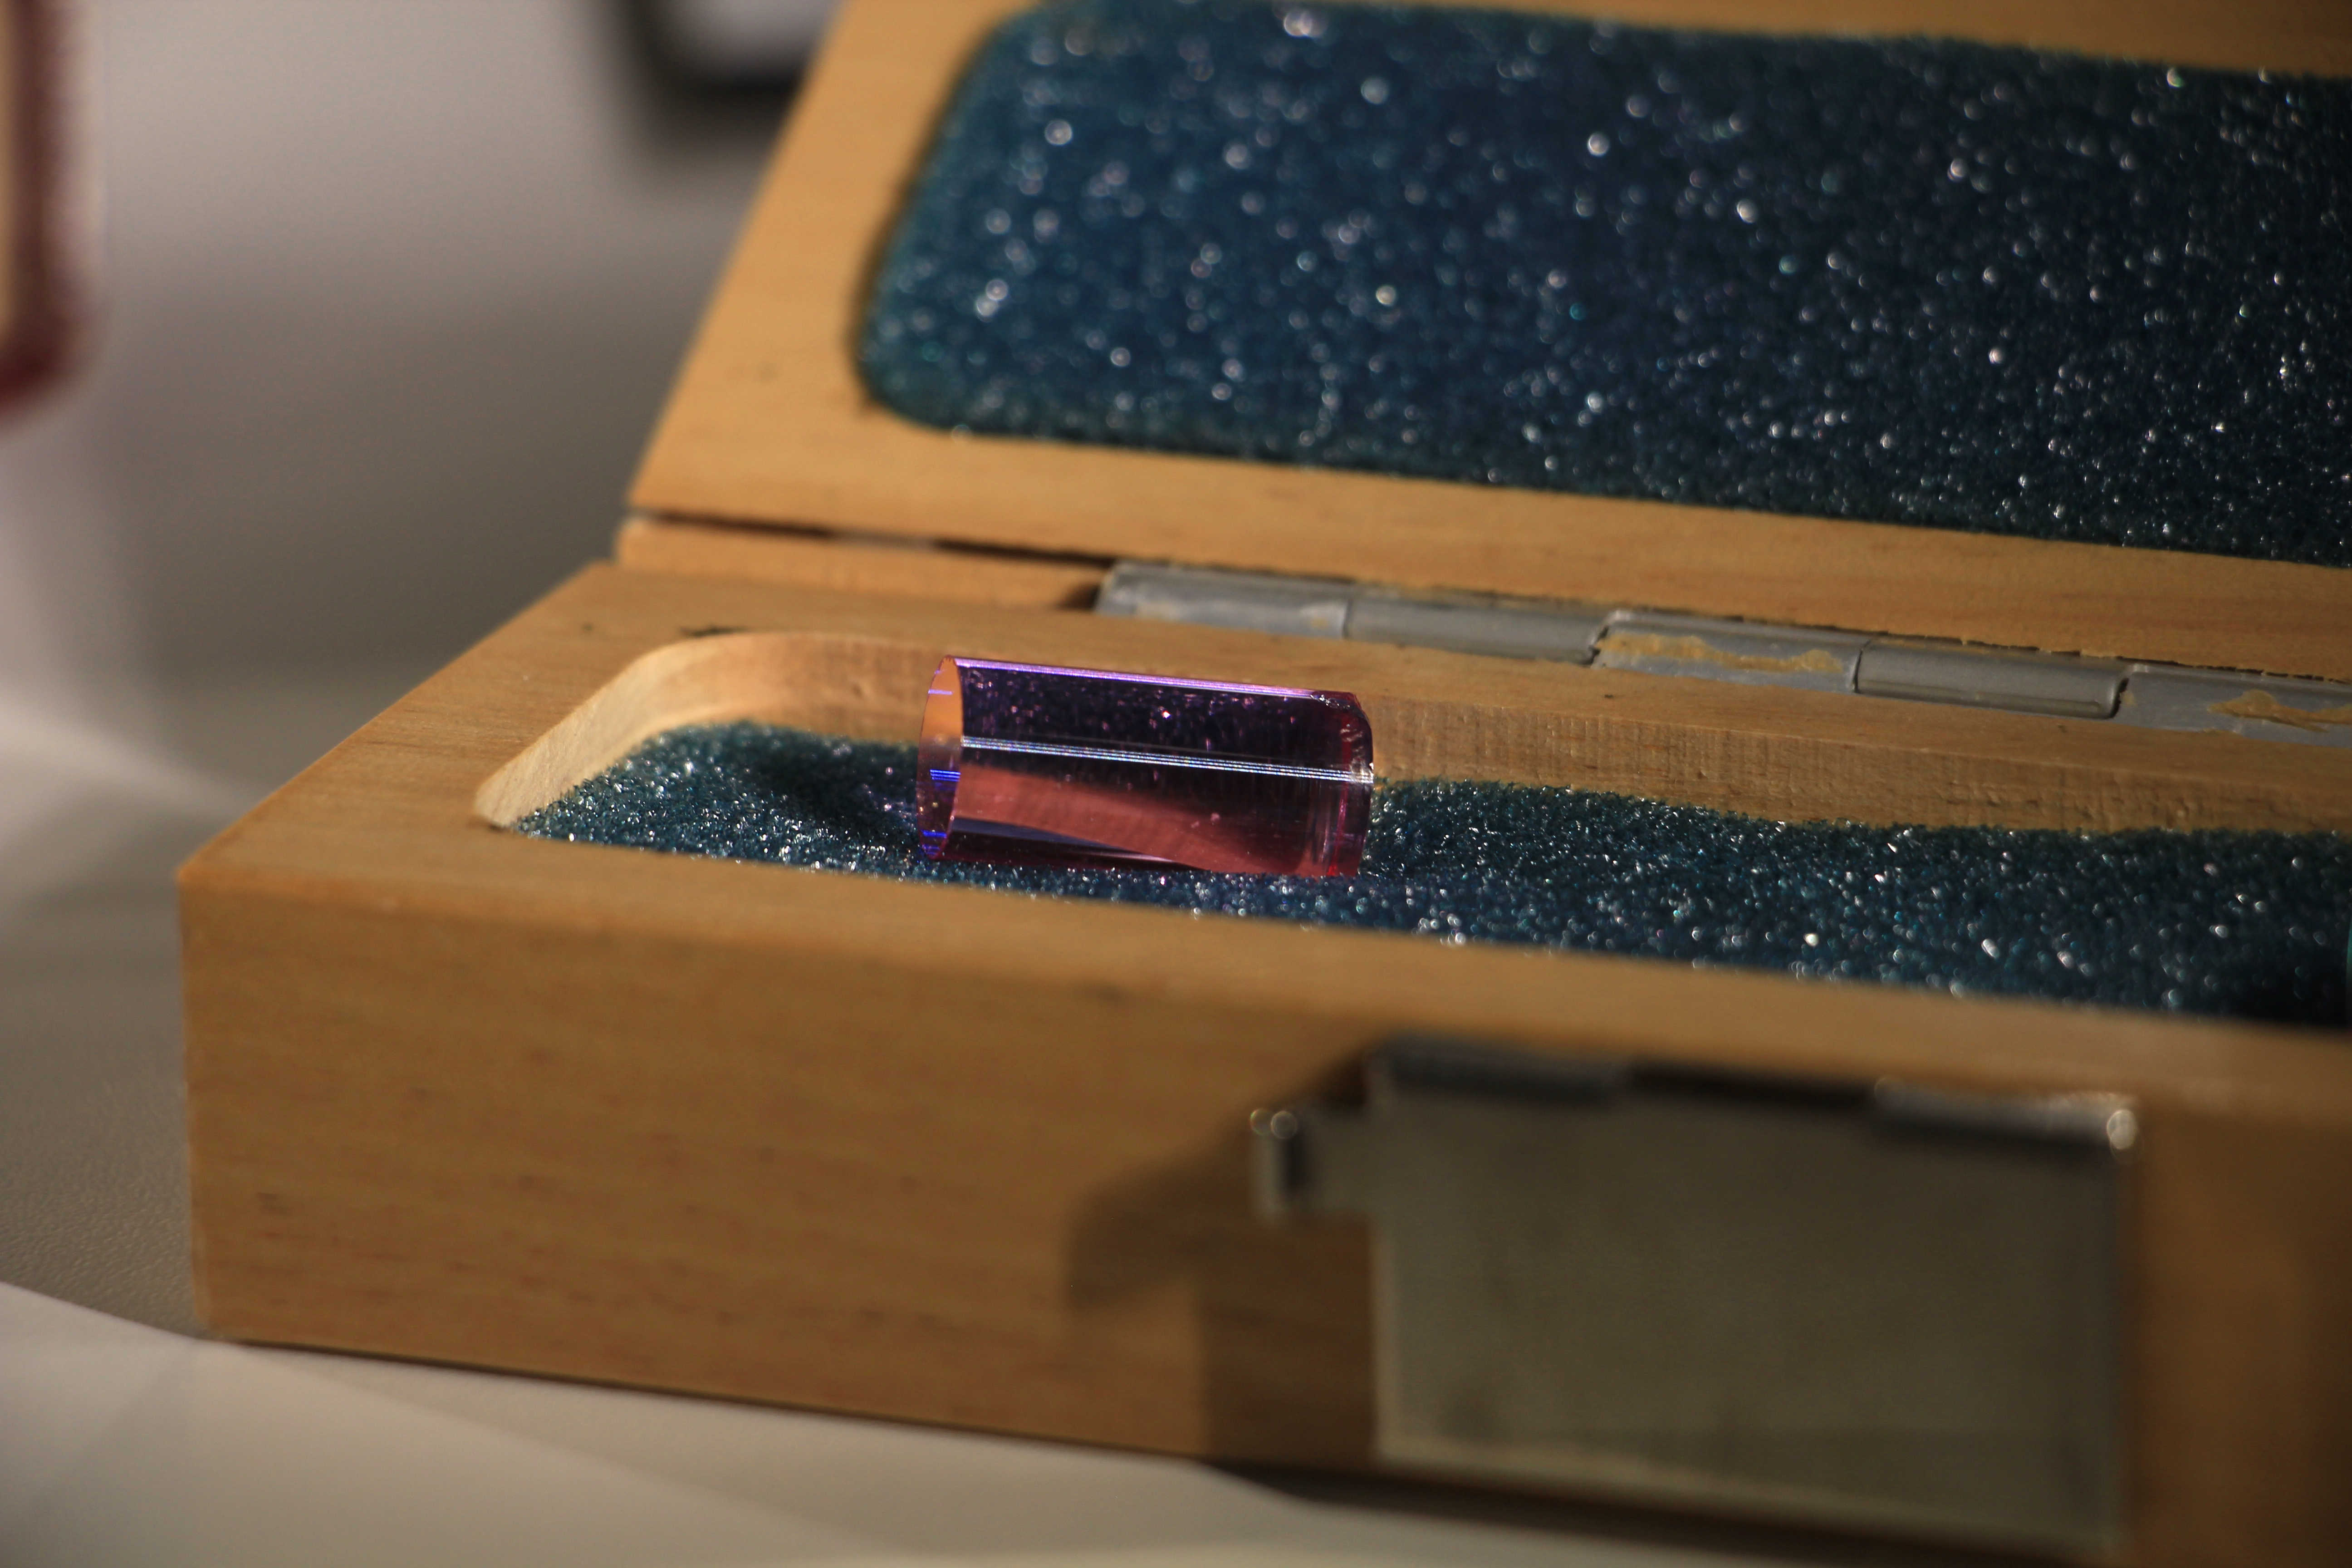
\includegraphics[width=\textwidth]{fig/conclusion/maiman_ruby}
	\caption*{The synthetic ruby crystal used by T. Maiman and colleagues in the first human-made laser. Taken by the author on a visit to the Max Planck Institute of Quantum Optics, Garching, Germany.}
	\end{figure*}

	\noindent  Just as James Watt could not comprehend how the development of resource extraction, mass production, and intercontinental transit would be spurred on by his steam engine, we too are surely blind to the world we {may} be building.
	It took two centuries for the largest steam turbine capacity to grow from the kilowatt to the gigawatt scale, but the intervening investment in industrial and information infrastructure tends to compress societal learning curves \cite{SmilEnergy}.
	Indeed, Claude Cohen-Tannoudji himself reflected that few expected Bose-Einstein condensation to follow so rapidly after the pioneering works of Chu, Phillips, and colleagues \cite{CTNote}.
	One readily doubts Theodore Maiman glimpsed the extent of modern scientific finesse in the first glint of laser light from his ruby crystal in 1960.
	Indeed, while `quantum technology' is a young term, its use has exploded since it was coined in the 1960s.
	One of the earliest uses of the term in print, in a US National Research Council report \cite{Isotopes69} on the needs and uses of separated stable isotopes in 1968, reads as a cautionary tale for the technological optimist:

	\bigskip
	\hfill
	\begin{minipage}{0.9\textwidth}
	\emph{``While it is dangerous to predict the future, the Committee strongly believes that our society is entering an era of nuclear and quantum technology, that will be different from that of the present which is based largely on nonquantum, non-nuclear science. The uses of separated isotopes in this new technology - beyond those envisioned and discussed above - will probably be multifold. Among the diverse uses that may beome important in the future are structural components of nuclear reactors and devices, industrial product labelling, measuring and controlling air pollution, and industrial process and product control."}
	\end{minipage}
	\bigskip
	% It is instructive to reflect on the efficiency of these machines as generators of quantum matter.
	% The mass input is X to produce Y condensed atoms and detect only 10\% of them.
	% The COP is complicated by the atom loss along the way but if we consider the change in energy of only the charge of atoms distilled to the BEC, then we find a COP of X.
	% The duty cycle of about 30mHz means that even with large BECs the average flux rate is only X.
	% These are low, but one would do well to recall that the first steam engines had efficiencies below 1\%, and several engineering breakthroughs later brought them towards several tens of percent, and gasoline engines followed a similar trend.
	% In the production of BEC in the new machine, the duty cycle is reduced by a factor of ten and the atom number by a factor of two, an increase in the time-coherence product of a factor of twenty.
	% Indeed, the characteristically quantum qualities of coherence and entanglemeent are being recast as quantifiable resources.
	
	
	\noindent The early decades of the 21st century {may} see the proliferation of cold-atom systems into wider application, following the path of the laser from R\&D to ubiquity.
	The children of 2121 {may} live in a world shaped as much by engineered quantum systems as today's society is by the repercussions of the first quantum revolution.
	They {may} look upon today's cold-atom machines as `primitive' in the same way that we look upon vaccum tubes and typewriters as quaint vestiges of a bygone era.
	We \emph{may} cross the precipice of the 21st century \cite{OrdPrecipice} and realize some of the innumerable possibilities bejeweling the vastness of Hilbert space.
	If we do, may we enjoy the burgeoning fruits of science with discerning wisdom and boundless generosity.
	After all - unlike the atoms in these experiments, we do not live in a vacuum.

	

\vfill

% \section*{Coda}	
\section*{\begin{figure*}[!h]
\centering
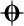
\includegraphics[scale=2]{fig/conclusion/Coda_sign}
\end{figure*}}

% \vspace{3cm}

	{Albert} Michelson may have lived to rue his proclamation at the inauguration of the Ryserson Physics Laboratory that `the great principles had already been discovered, and that physics would henceforth be limited to finding truths in the sixth decimal place.'
	Nobody could repeat this mistake today as we can readily identify subjects awaiting clear insight, such as the nature of dark matter and dark energy, or the synthesis of quantum field theory and general relativity.
	At first glance, the dogged pursuit of the next digit of precision could appear a peculiar lens with which to bring such quandaries into focus, and one could demur the endeavour as searching for a revolution in the margins of Nature.
	But surely such an enterprise would find vindication in a discovery that the fundamental constants were contingent, in deciding whether or not gravity is fundamentally quantum, or in establishing control of dark matter?
	Albert Einstein, on whose shoulders this work squarely rests, noted that a well-formulated question contains its own answer. 
	Although we can't be sure from the side of the revolution, perhaps we are beginning to ask the right questions.
	
\vfill	

\begin{center}
\vfill
\singlespacing
\emph{``The key to discoveries is to look at those\\
 places where there is still a paradox.\\
It’s like the tip of an iceberg.\\
If there is a point of \\
dissatisfaction, \\
take a closer \\
look at it.'' \\-\\
\emph{Edral Arikan}}
 \end{center}


 



	




% \section*{Scraps}


%Was lured in to the academy by the promise of
% questions like `what is the difference between simplicity and
% complexity' - when are things simple? When is something intrinsically
% hard to represent, even if it exists effortlessly in its own right? This
% drew me to lattice - to build something with the hands that would be so
% elusive for theory and computing.


% 	But let us not lose sight of the implicit `right to know' - that
% we still embody the notion of a conquest over nature, of mastery of the
% other, the greater, the ultimately incomprehensible.
% 	Let us not fall
% victim to our own arrogances, and recall that in our turbulent times,
% our investigations come at cost.
% 	This remains ingrained in our
% mythology - that more advanced technology is always worth the price that
% is paid.
% 	In the limit of free, clean energy and post-scarcity
% manufacture whereby human labour is eliminated, this may be true.
	






% Schrodinger quote goes here?


% Notes on some other dissertation conclusions
	


% % 	Davis, Dynamics of BEC

% % 	Greiner, ultracold gases in 3D lattices 375 wds
% 	2 page outlook
% 	Open questions answerable with the present system
% 	POssible extensions (eg fermionic lattice, photoassociation, non-BH hamiltonians, vortices, spin-dependent lattices)

% % 	Schneider, interacting fermions 2 pages
% 	One para main topic
% 	One para per three experiments
% 	One para possible issues and improvements
% 	Outlook
% 		A few directions for future research and what the lab is up to


% % 	Bakr, Microscopic QPTs 5 pages double spaced
% 	No conclusion, each chapter self contained
% 	Outlook chapter instead
% 	Roughly one para per suggested direction or improvement


% % 	Hodgman, lifetime & correlation measurements 506 wds
% 	Summary 2 pages
% 		One para summarizing transition works
% 		One para detailing new PAL method
% 		One para on distinguishing thermal and coherent clouds
% 		Couple paragraphs extended summary of a particular experiment
% 	Future work
% 		2 pages inc big figure
% 		Identify a couple transitions whose rates could be measured
% 		Other applications of correlation funs
% 		A couple big-ticket items (EPR for massive particles)

% % 	Struck, Artificial gauge fields 
% 	Each chapter has own conclusion and outlook


% % 	Aidelsburger, artificial gauge fields 
% 	1.5 pages conc
% 		The main topic was...
% 		Summary of the subject and findings of each major chapter

% 	1.5 outlook
% 		Issues and improvements on experiments
% 		A couple incremental steps forward

% % 	Izaac, continuous-time quantum walks 
% 	Most chapters have their own conclusion
% 	3.5 page conclusion
% 	One (big) paragraph of detailed summary of each chapter
% 	Unanswered questions, possible applications of the theory, and a speculative forward-looking paragraph
% 		'we are yet to scratch the surface of what quantum walks are capable of'


% % 	Lukin, entanglement in 1D 341 wds
% 	Super short thesis. 2 page conclusion
% 	In this thesis (summary of major results)
% 	one para summary of major works: Technique, finding, implication
% 	A couple of possible extensions of the apparatus

% % 	Phelps, dipolar QGM 
% 	6.5 pages double space
% 	OUtstanding challenges 
% 	Three sections, 3-5 para each, with potential future directions. 


% % 	Shin, Nonlocal correlations
% 	3 page conclusion
% 	One para summary of thesis contents
% 	3 sections, 3-4 paragraphs on possible research topics
